\documentclass{article}
\title{CS 205 Homework 5}
\author{Keith Lehman, kpl56@scarletmail.rutgers.edu}

\usepackage[margin=0.5in]{geometry}
\usepackage{graphicx}
\usepackage{amssymb}

\begin{document}
\maketitle

\begin{enumerate}

\item Given an arbitrary relation $R$, suppose we compute two new relations. Prove $R_{1} = R_{2}$ for all $R$. \\
For $R_{1}$ to be the reflixive closure of the transitive closure of $R$, it first must have every element map to the next element and every succeeding element. For it to be reflexive, each element mentioned must also be related to itself. For $R_{2}$ to be the transitive closure of the reflexive closure of $R$, it first must have every element related to itself, then, for each element, it must relate to the following element, as well as every other following element. Under these conditions, both $R_{1}$ and $R_{2}$ will continue the exact same elements. 

\item Let $ A = $ \{cat, dog, bird, rat\} and $R$ be a relation on $A$ defined by \{$(x,y): x$ and $y$ have at least one letter in common\}. \\
\begin{enumerate}
    \item  Draw $R$ as a directed graph. \\
    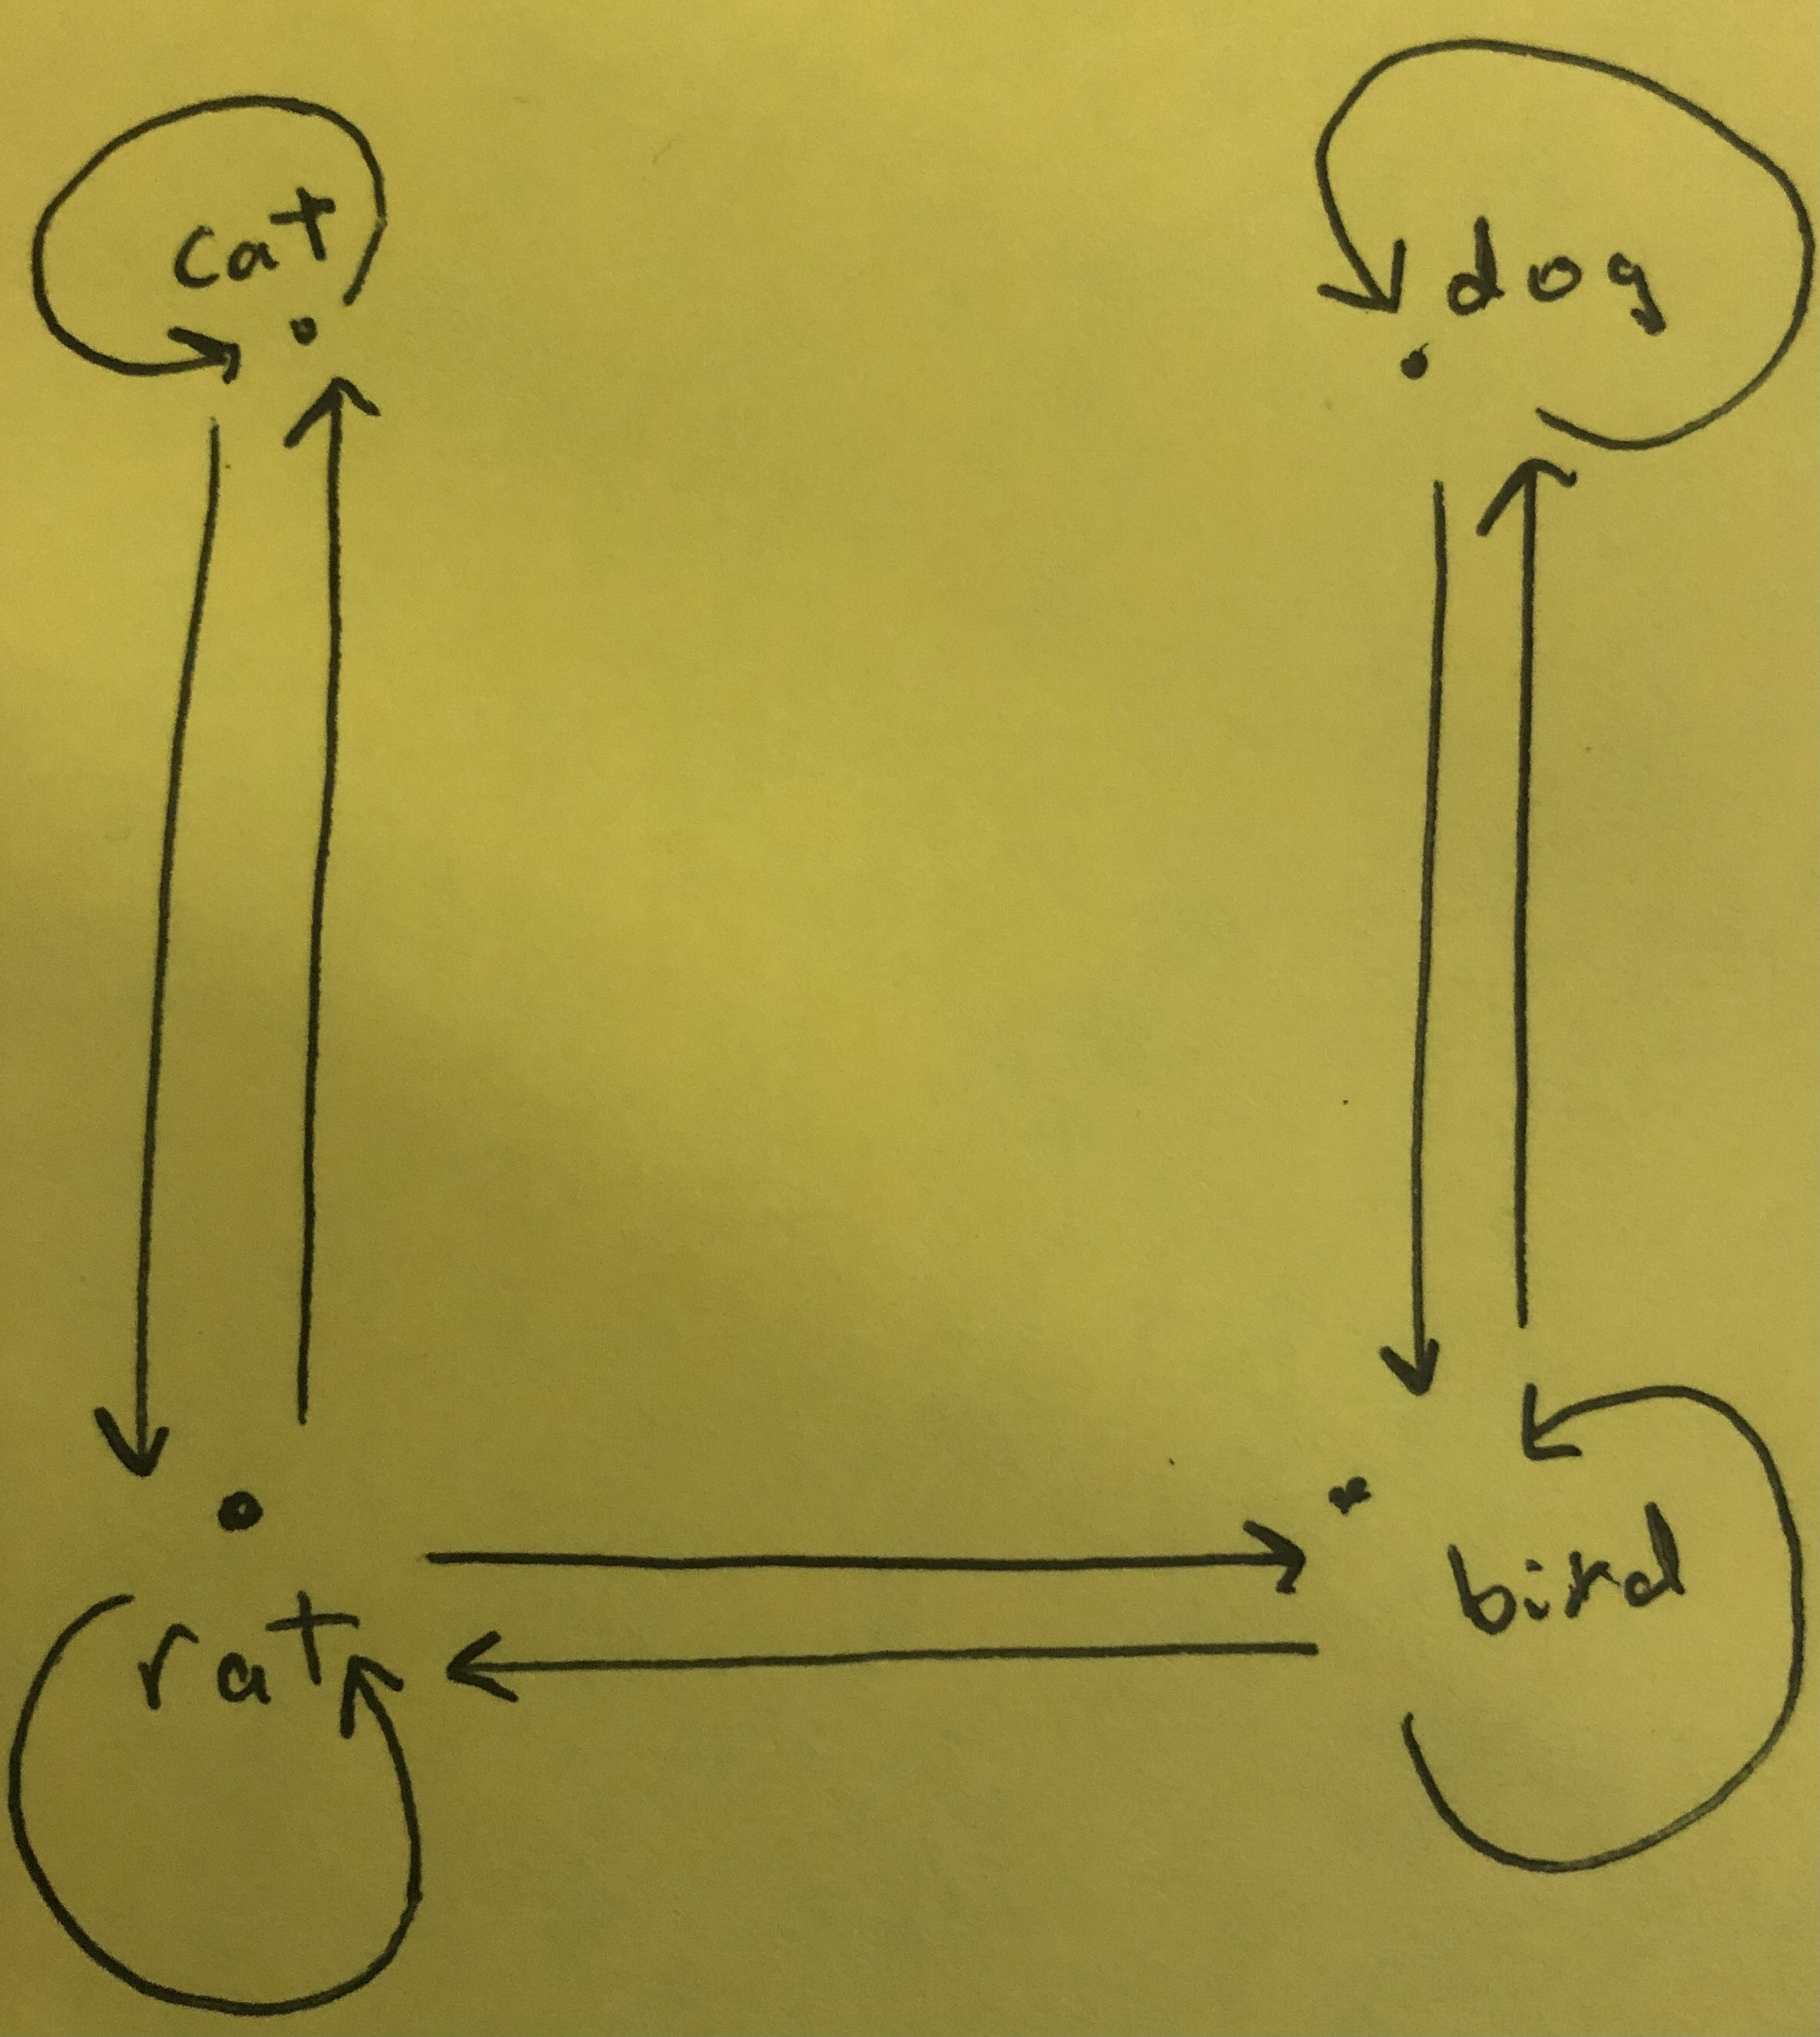
\includegraphics[scale=0.05]{image0.jpg}
    \item  Is $R$ reflexive, symmetric, and/or transitive? \\
    $R$ is reflexive as every element has every letter in common with itself. $R$ is also symmetric because if one element has a letter in common with another element, that other element also has that same letter in common with the first. $R$ is NOT transitive. While element 1 may have a letter in common with element 2 and element 2 might have a letter in common with element 3, these could be different letters meaning that element 1 may not be related to element 3, making it NOT transitive.
\end{enumerate}

\item Given a relation $R$ on a set $A$, prove that if $R$ is transitive, then so is $R^{-1}$. \\
For $R$ to be transitive on set $A$, substituting indexes for elements, $R$ must contain \{$(0,1),(1,2),(2,3)..(n,n+1),(0,n+1)$\}. Therefore, we know that $R^{-1}$ must contain \{$(n+1,n)..(3,2),(2,1),(1,0),(n+1,0)$\}. While in a different order, the first element is still related to the last, making the entire relation transitive. 

\item Suppose $R$ and $S$ are symmetric relations on a set $A$. Prove that $R \circ S $ is symmetric iff $R \circ S = S \circ R$.
\end{enumerate}
\end{document}
